\documentclass[a4paper,11pt]{article}

\usepackage[utf8]{inputenc}
\usepackage[T1]{fontenc}
\usepackage{geometry}
\geometry{margin=20mm, top=25mm, bottom=25mm}
\usepackage{tikz}
\usetikzlibrary{patterns, arrows.meta, decorations.markings, calc, positioning, angles, quotes}
\usepackage{siunitx}
\sisetup{per-mode=symbol}
\usepackage{booktabs}
\usepackage{array}
\usepackage{xcolor}
\usepackage{fancyhdr}
\usepackage{amsmath}
\usepackage{enumitem}
\usepackage{tabularx}
\usepackage{float}
\usepackage{pgfplots}
\pgfplotsset{compat=1.18}
\usepackage{lastpage}

% Couleurs
\definecolor{cotbleu}{HTML}{2563EB}
\definecolor{cotrouge}{HTML}{DC2626}
\definecolor{cotvert}{HTML}{16A34A}
\definecolor{graphitegris}{HTML}{4B5563}
\definecolor{coneint}{HTML}{F59E0B}
\definecolor{fondgris}{HTML}{F3F4F6}
\definecolor{photon}{HTML}{E97316}
\definecolor{cuivre}{HTML}{B45309}

\pagestyle{fancy}
\fancyhf{}
\lhead{\small\textsc{Loupe Compton --- Assemblage optimal}}
\rhead{\small Calcul g\'eom\'etrique}
\cfoot{\thepage/\pageref{LastPage}}
\renewcommand{\headrulewidth}{0.4pt}

\title{%
  \vspace{-1cm}
  {\Large\textsc{Assemblage Optimal}}\\[4pt]
  {\LARGE\bfseries Loupe Compton --- C\^one Graphite}\\[4pt]
  {\large Source quasi-ponctuelle, c\^one d'\'emission $2\alpha_s = 60°$, spectre 10--50\,keV}
}
\author{}
\date{F\'evrier 2026}

\begin{document}
\maketitle
\thispagestyle{fancy}

% ============================================================
\section{Mod\`ele de source et g\'eom\'etrie}
% ============================================================

\subsection{Param\`etres de la source}

\begin{table}[H]
\centering
\begin{tabular}{@{}ll@{}}
\toprule
\textbf{Param\`etre} & \textbf{Valeur} \\
\midrule
Type            & Source quasi-ponctuelle (Amptek MiniX) \\
Spectre         & Continu, 10 \`a \SI{50}{\keV} \\
C\^one d'\'emission & $2\alpha_s = 60°$ (demi-angle $\alpha_s = 30°$) \\
Distribution    & Suppos\'ee uniforme dans le c\^one \\
\bottomrule
\end{tabular}
\end{table}

\subsection{Param\`etres du c\^one concentrateur}

\begin{table}[H]
\centering
\begin{tabular}{@{}ll@{}}
\toprule
\textbf{Param\`etre} & \textbf{Valeur} \\
\midrule
Rayon ext\'erieur $R_{\text{ext}}$   & \SI{25}{\mm} (diam\`etre \SI{50}{\mm}) \\
Rayon int\'erieur entr\'ee $R_{\text{in}}$ & \SI{5}{\mm} (diam\`etre \SI{10}{\mm}) \\
Rayon int\'erieur sortie $R_{\text{out}}$  & \SI{1.5}{\mm} (diam\`etre \SI{3}{\mm}) \\
Longueur $L$                     & \SI{40}{\mm} \\
Demi-angle interne $\alpha_c$     & $\arctan\!\Big(\frac{5 - 1{,}5}{40}\Big) = 5{,}0°$ \\
\bottomrule
\end{tabular}
\end{table}

% ============================================================
\section{Calcul de la distance optimale source--entr\'ee}
% ============================================================

\subsection{G\'eom\'etrie du probl\`eme}

\begin{figure}[H]
\centering
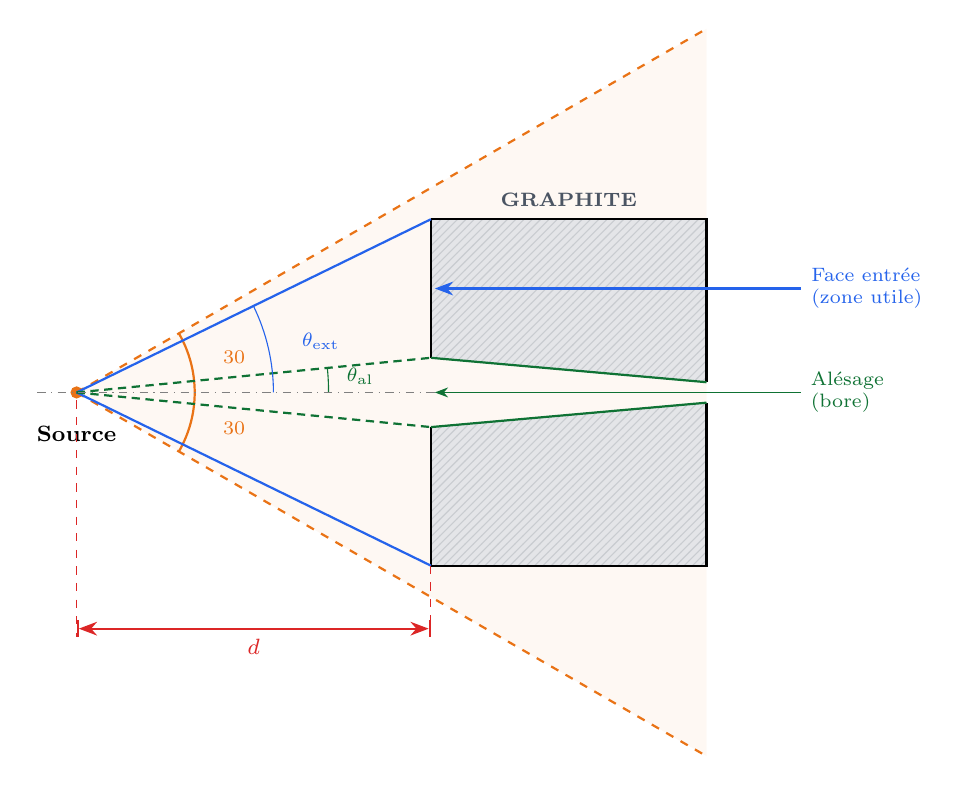
\begin{tikzpicture}[>=Stealth, scale=1.0, every node/.style={font=\small}]

  % Source
  \filldraw[photon] (0,0) circle (2pt);
  \node[below, font=\footnotesize\bfseries] at (0,-0.3) {Source};

  % Cone d'émission
  \draw[photon, thick, dashed] (0,0) -- (8, {8*tan(30)});
  \draw[photon, thick, dashed] (0,0) -- (8, {-8*tan(30)});
  \fill[photon, opacity=0.05] (0,0) -- (8, {8*tan(30)}) -- (8, {-8*tan(30)}) -- cycle;

  % Angle d'émission
  \draw[photon, thick] (1.5,0) arc[start angle=0, end angle=30, radius=1.5];
  \draw[photon, thick] (1.5,0) arc[start angle=0, end angle=-30, radius=1.5];
  \node[photon, font=\scriptsize] at (2.0, 0.45) {$30°$};
  \node[photon, font=\scriptsize] at (2.0, -0.45) {$30°$};

  % Distance d
  \pgfmathsetmacro{\d}{4.5}  % distance source-entrée (en cm sur le dessin)
  
  % Graphite cone (simplifié)
  \pgfmathsetmacro{\Lc}{3.5}
  \pgfmathsetmacro{\Rc}{2.2}
  \pgfmathsetmacro{\Ric}{0.44}
  \pgfmathsetmacro{\Roc}{0.13}
  
  \begin{scope}[shift={(\d,0)}]
    % Corps
    \fill[graphitegris!15] (0,\Ric) -- (0,\Rc) -- (\Lc,\Rc) -- (\Lc,\Roc) -- cycle;
    \fill[graphitegris!15] (0,-\Ric) -- (0,-\Rc) -- (\Lc,-\Rc) -- (\Lc,-\Roc) -- cycle;
    \fill[pattern=north east lines, pattern color=graphitegris!30] 
      (0,\Ric) -- (0,\Rc) -- (\Lc,\Rc) -- (\Lc,\Roc) -- cycle;
    \fill[pattern=north east lines, pattern color=graphitegris!30] 
      (0,-\Ric) -- (0,-\Rc) -- (\Lc,-\Rc) -- (\Lc,-\Roc) -- cycle;
    \draw[thick] (0,\Rc) -- (\Lc,\Rc) -- (\Lc,\Roc);
    \draw[thick] (0,-\Rc) -- (\Lc,-\Rc) -- (\Lc,-\Roc);
    \draw[thick] (0,\Rc) -- (0,\Ric);
    \draw[thick] (0,-\Rc) -- (0,-\Ric);
    \draw[thick, cotvert!70!black] (0,\Ric) -- (\Lc,\Roc);
    \draw[thick, cotvert!70!black] (0,-\Ric) -- (\Lc,-\Roc);
    
    % Labels
    \node[graphitegris, font=\scriptsize\bfseries] at ({\Lc/2},{\Rc+0.25}) {GRAPHITE};
  \end{scope}

  % Angles subtendus
  \draw[cotbleu, thick] (0,0) -- ({\d},\Rc);
  \draw[cotbleu, thick] (0,0) -- ({\d},-\Rc);
  \draw[cotvert!70!black, thick, densely dashed] (0,0) -- ({\d},\Ric);
  \draw[cotvert!70!black, thick, densely dashed] (0,0) -- ({\d},-\Ric);

  % Theta labels
  \draw[cotbleu] (2.5,0) arc[start angle=0, end angle={atan(\Rc/\d)}, radius=2.5];
  \node[cotbleu, font=\scriptsize] at (3.1, 0.65) {$\theta_{\text{ext}}$};
  
  \draw[cotvert!70!black] (3.2,0) arc[start angle=0, end angle={atan(\Ric/\d)}, radius=3.2];
  \node[cotvert!70!black, font=\scriptsize] at (3.6, 0.2) {$\theta_{\text{al}}$};

  % Distance d
  \draw[cotrouge, |<->|, thick] (0,-3.0) -- node[below, font=\footnotesize\bfseries, cotrouge] {$d$} (\d,-3.0);
  \draw[cotrouge, thin, dashed] (0,-0.1) -- (0,-3.1);
  \draw[cotrouge, thin, dashed] (\d, -\Rc) -- (\d,-3.1);

  % Axe
  \draw[dash dot, thin, gray] (-0.5,0) -- ({\d+\Lc+0.5},0);

  % Zones annotées
  \draw[<-, cotbleu, thick] ({\d+0.05}, {(\Rc+\Ric)/2}) -- ({\d+\Lc+1.2}, {(\Rc+\Ric)/2}) 
    node[right, font=\scriptsize, cotbleu, align=left] {Face entr\'ee\\(zone utile)};
  \draw[<-, cotvert!70!black] ({\d+0.05}, 0) -- ({\d+\Lc+1.2}, 0) 
    node[right, font=\scriptsize, cotvert!70!black, align=left] {Al\'esage\\(bore)};

\end{tikzpicture}
\caption{G\'eom\'etrie source--c\^one. Le faisceau conique de demi-angle $\alpha_s = 30°$ illumine l'entr\'ee du c\^one \`a distance $d$. Les photons dans l'angle $\theta_{\text{al}}$ traversent l'al\'esage (bore) ; ceux entre $\theta_{\text{al}}$ et $\theta_{\text{ext}}$ frappent la face en graphite.}
\label{fig:geometrie}
\end{figure}

\subsection{Angles subtendus}

\`A distance $d$ de la source, le c\^one subtend deux demi-angles :
\begin{align}
  \theta_{\text{ext}} &= \arctan\!\left(\frac{R_{\text{ext}}}{d}\right) = \arctan\!\left(\frac{25}{d}\right) \label{eq:theta_ext} \\[4pt]
  \theta_{\text{al}} &= \arctan\!\left(\frac{R_{\text{in}}}{d}\right) = \arctan\!\left(\frac{5}{d}\right) \label{eq:theta_bore}
\end{align}

\subsection{Cat\'egories de photons}

Pour une source \'emettant uniform\'ement dans un c\^one de demi-angle $\alpha_s = 30°$, l'angle solide total est :
\begin{equation}
  \Omega_s = 2\pi\,(1 - \cos\alpha_s) = 2\pi\,(1 - \cos 30°) \approx 0{,}842\;\text{sr}
\end{equation}

Les photons se r\'epartissent en trois cat\'egories :

\medskip
\noindent\textbf{1. Photons frappant la face en graphite} ($\theta_{\text{al}} < \theta < \min(\theta_{\text{ext}},\, \alpha_s)$)~:
\begin{equation}
  \eta_{\text{face}} = \frac{\cos\theta_{\text{al}} - \cos\!\big(\min(\theta_{\text{ext}},\, 30°)\big)}{1 - \cos 30°}
  \label{eq:eta_face}
\end{equation}

\noindent\textbf{2. Photons entrant dans l'al\'esage} ($0 < \theta < \theta_{\text{al}}$)~:
\begin{equation}
  \eta_{\text{bore}} = \frac{1 - \cos\theta_{\text{al}}}{1 - \cos 30°}
  \label{eq:eta_bore}
\end{equation}

\noindent\textbf{3. Photons perdus} ($\theta > \theta_{\text{ext}}$ ou $\theta > 30°$)~:
\begin{equation}
  \eta_{\text{perdu}} = 1 - \eta_{\text{face}} - \eta_{\text{bore}}
  \label{eq:eta_perdu}
\end{equation}

\subsection{R\'esultats num\'eriques}

\begin{table}[H]
\centering
\caption{Efficacit\'e g\'eom\'etrique en fonction de la distance $d$. La figure de m\'erite est $\text{FoM} = \eta_{\text{face}} \times P_C^{\text{fwd}}$ (avec $P_C^{\text{fwd}} = 20{,}6\,\%$).}
\label{tab:distances}
\renewcommand{\arraystretch}{1.3}
\begin{tabular}{@{} r r r r r r r @{}}
\toprule
$d$ & $\theta_{\text{ext}}$ & $\theta_{\text{al}}$ & $\eta_{\text{face}}$ & $\eta_{\text{bore}}$ & $\eta_{\text{perdu}}$ & FoM \\
(mm) & (deg) & (deg) & (\%) & (\%) & (\%) & (\%) \\
\midrule
20 & 51{,}3 & 14{,}0 & 77{,}6 & 22{,}4 & 0{,}0\rlap{$^{*}$} & 16{,}0 \\
25 & 45{,}0 & 11{,}3 & 85{,}3 & 14{,}7 & 0{,}0\rlap{$^{*}$} & 17{,}6 \\
30 & 39{,}8 & 9{,}5 & 89{,}8 & 10{,}2 & 0{,}0\rlap{$^{*}$} & 18{,}5 \\
35 & 35{,}5 & 8{,}1 & 92{,}6 & 7{,}4 & 0{,}0\rlap{$^{*}$} & 19{,}1 \\
40 & 32{,}0 & 7{,}1 & 93{,}8 & 5{,}7 & 0{,}5 & 19{,}3 \\
\textbf{43} & \textbf{30{,}2} & \textbf{6{,}6} & \textbf{95{,}1} & \textbf{4{,}9} & \textbf{0{,}0} & \textbf{19{,}6} \\
45 & 29{,}1 & 6{,}3 & 93{,}4 & 4{,}5 & 2{,}1 & 19{,}2 \\
50 & 26{,}6 & 5{,}7 & 89{,}3 & 3{,}7 & 7{,}0 & 18{,}4 \\
60 & 22{,}6 & 4{,}8 & 80{,}7 & 2{,}6 & 16{,}7 & 16{,}6 \\
\bottomrule
\multicolumn{7}{@{}l}{\footnotesize $^{*}$ \`A $d < 43$\,mm, le faisceau d\'eborde du diam\`etre ext\'erieur : $\eta_{\text{perdu}} = 0$ mais $\theta_{\text{ext}}$ est tronqu\'e \`a $30°$.}
\end{tabular}
\end{table}

\begin{figure}[H]
\centering
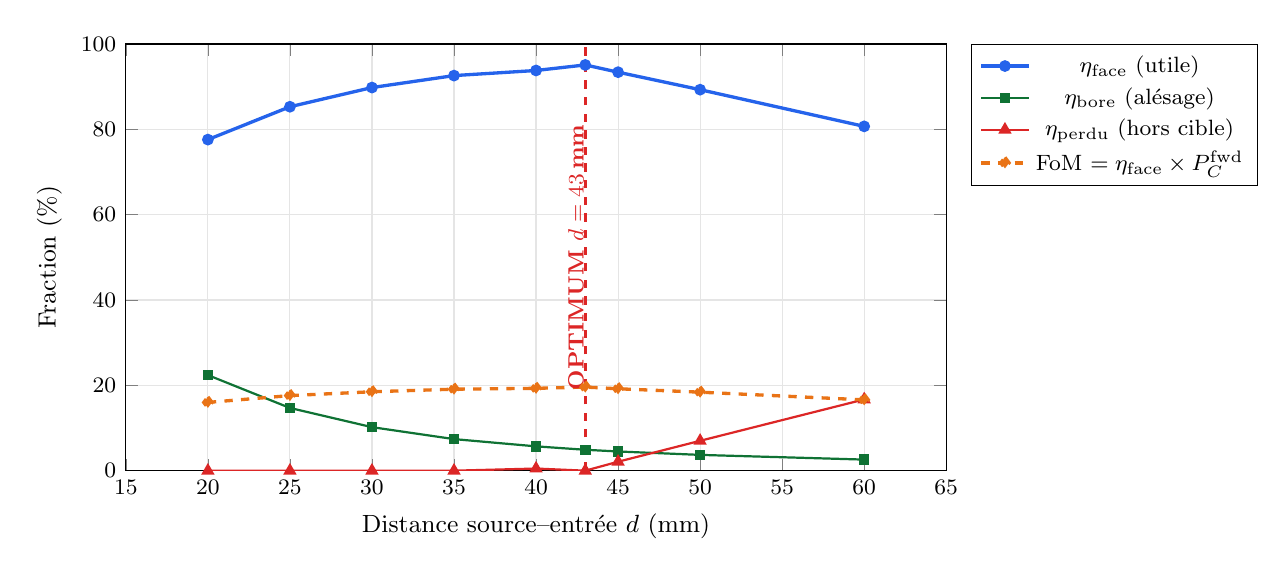
\begin{tikzpicture}
\begin{axis}[
  width=12cm, height=7cm,
  xlabel={Distance source--entr\'ee $d$ (mm)},
  ylabel={Fraction (\%)},
  xmin=15, xmax=65,
  ymin=0, ymax=100,
  grid=major,
  grid style={gray!20},
  legend pos=outer north east,
  legend style={font=\footnotesize},
  every axis label/.style={font=\small},
  tick label style={font=\footnotesize},
]

% eta_face
\addplot[cotbleu, very thick, mark=*, mark size=1.5pt] coordinates {
  (20,77.6) (25,85.3) (30,89.8) (35,92.6) (40,93.8) (43,95.1) (45,93.4) (50,89.3) (60,80.7)
};
\addlegendentry{$\eta_{\text{face}}$ (utile)}

% eta_bore
\addplot[cotvert!70!black, thick, mark=square*, mark size=1.5pt] coordinates {
  (20,22.4) (25,14.7) (30,10.2) (35,7.4) (40,5.7) (43,4.9) (45,4.5) (50,3.7) (60,2.6)
};
\addlegendentry{$\eta_{\text{bore}}$ (al\'esage)}

% eta_perdu
\addplot[cotrouge, thick, mark=triangle*, mark size=2pt] coordinates {
  (20,0) (25,0) (30,0) (35,0) (40,0.5) (43,0) (45,2.1) (50,7.0) (60,16.7)
};
\addlegendentry{$\eta_{\text{perdu}}$ (hors cible)}

% FoM (scaled x5 for visibility)
\addplot[photon, very thick, dashed, mark=diamond*, mark size=2pt] coordinates {
  (20,16.0) (25,17.6) (30,18.5) (35,19.1) (40,19.3) (43,19.6) (45,19.2) (50,18.4) (60,16.6)
};
\addlegendentry{FoM $= \eta_{\text{face}} \times P_C^{\text{fwd}}$}

% Optimum marker
\draw[cotrouge, very thick, dashed] (axis cs:43,0) -- (axis cs:43,100);
\node[cotrouge, font=\footnotesize\bfseries, rotate=90, anchor=south] at (axis cs:43.5,50) {OPTIMUM $d = 43$\,mm};

\end{axis}
\end{tikzpicture}
\caption{Efficacit\'e g\'eom\'etrique en fonction de la distance $d$. L'optimum est \`a $d \approx \SI{43}{\mm}$ o\`u $\eta_{\text{face}} = 95{,}1\,\%$ et la FoM atteint son maximum.}
\label{fig:eta_vs_d}
\end{figure}

\subsection{Condition d'optimalit\'e}

L'optimum correspond \`a la distance o\`u le bord ext\'erieur du faisceau co\"incide exactement avec le bord ext\'erieur de la pi\`ece :
\begin{equation}
  \boxed{d^* = \frac{R_{\text{ext}}}{\tan\alpha_s} = \frac{25}{\tan 30°} = \frac{25}{0{,}577} \approx \SI{43.3}{\mm}}
  \label{eq:d_opt}
\end{equation}

\`A cette distance :
\begin{itemize}[itemsep=2pt]
  \item 95{,}1\,\% des photons frappent la face en graphite (zone utile).
  \item 4{,}9\,\% traversent l'al\'esage (une partie frappe la paroi interne du c\^one).
  \item 0\,\% sont perdus hors cible.
\end{itemize}

% ============================================================
\section{Contribution des photons de l'al\'esage}
% ============================================================

Les 4{,}9\,\% de photons entrant dans l'al\'esage ne sont pas tous perdus. Un photon entrant \`a rayon $r < R_{\text{in}}$ avec un angle $\theta$ par rapport \`a l'axe frappe la paroi conique interne \`a la distance :
\begin{equation}
  z_{\text{impact}} = \frac{R_{\text{in}} - r}{\tan\theta + \tan\alpha_c}
\end{equation}

o\`u $\alpha_c = 5°$ est le demi-angle du c\^one interne. \`A $d = 43$\,mm, les angles vont de $0$ \`a $\theta_{\text{al}} = 6{,}6°$. Le tableau suivant donne quelques exemples :

\begin{table}[H]
\centering
\caption{Impact des photons de bore sur la paroi conique interne ($d = 43$\,mm, $r = 0$ -- axe).}
\label{tab:bore}
\renewcommand{\arraystretch}{1.2}
\begin{tabular}{@{} r r r r @{}}
\toprule
$\theta$ (deg) & $z_{\text{impact}}$ (mm) & \'Epaisseur travers\'ee & Interaction ? \\
\midrule
1 & 38{,}3 & $\sim 22$\,mm (rasant) & Oui, Compton probable \\
3 & 33{,}0 & $\sim 18$\,mm (rasant) & Oui, Compton probable \\
5 & 25{,}3 & $\sim 12$\,mm & Compton possible \\
6{,}6 & 19{,}6 & $\sim 8$\,mm & Compton faible \\
\bottomrule
\end{tabular}
\end{table}

Environ la moiti\'e des photons du bore ($\sim 2{,}5\,\%$ du total) subissent une interaction Compton dans la paroi interne. Cela ajoute $\sim 0{,}5\,\%$ au rendement total. L'effet est modeste mais positif.

% ============================================================
\section{Placement du filtre Cu}
% ============================================================

Le filtre Cu \SI{25}{\micro\meter} doit \^etre plac\'e le plus pr\`es possible de la source pour deux raisons :
\begin{enumerate}[itemsep=2pt]
  \item \textbf{Minimiser la divergence \`a la travers\'ee :} un filtre proche couvre un faisceau encore \'etroit, r\'eduisant la taille de filtre n\'ecessaire.
  \item \textbf{\'Eliminer les basses \'energies avant qu'elles n'interagissent :} les photons $< 15$\,keV doivent \^etre absorb\'es \emph{avant} le graphite, sinon ils sont absorb\'es par effet photo\'electrique dans le c\^one (inutile et source de fluorescence parasite).
\end{enumerate}

\begin{table}[H]
\centering
\caption{Position du filtre et diam\`etre utile requis.}
\renewcommand{\arraystretch}{1.2}
\begin{tabular}{@{} r r l @{}}
\toprule
$d_{\text{filtre}}$ (mm) & $\varnothing_{\text{utile}}$ (mm) & Remarque \\
\midrule
2 & $2 \times 2\,\tan 30° = 2{,}3$ & Tr\`es compact, id\'eal \\
\textbf{3} & \textbf{3{,}5} & \textbf{Recommand\'e (marge pratique)} \\
5 & 5{,}8 & Acceptable \\
10 & 11{,}5 & Filtre plus grand, co\^ut l\'eg\`erement sup\'erieur \\
\bottomrule
\end{tabular}
\end{table}

\textbf{Recommandation :} $d_{\text{filtre}} = \SI{3}{\mm}$ de la source. Le filtre peut \^etre un disque de Cu de $\varnothing\,\SI{6}{\mm}$ (marge) mont\'e sur un anneau support en plastique.

% ============================================================
\section{Plan d'assemblage optimal}
% ============================================================

\begin{figure}[H]
\centering
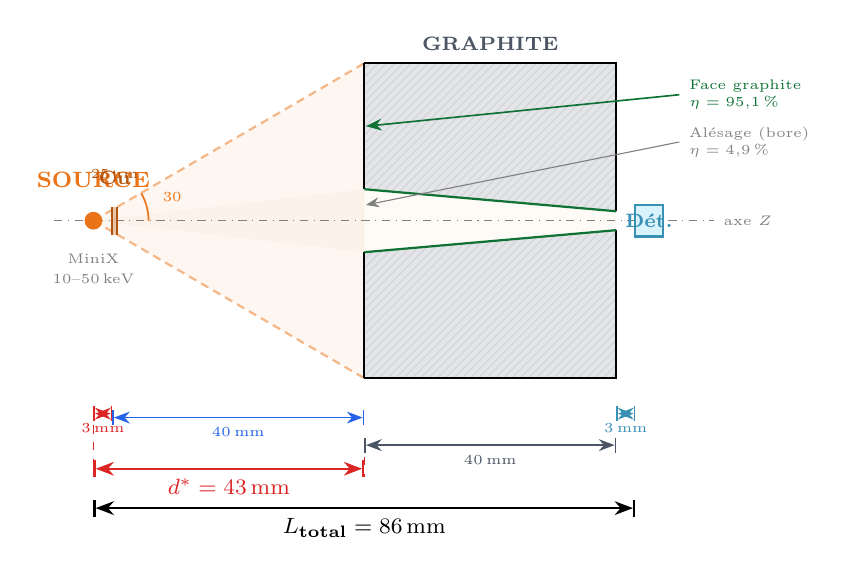
\begin{tikzpicture}[>=Stealth, scale=1.0, every node/.style={font=\small}]

  % === ECHELLE : 1mm = 0.08 cm ===
  \pgfmathsetmacro{\s}{0.08}
  
  % Positions (en mm réels -> cm dessin)
  \pgfmathsetmacro{\xS}{0}           % source
  \pgfmathsetmacro{\xF}{3*\s}        % filtre à 3mm
  \pgfmathsetmacro{\xC}{43*\s}       % entrée cône à 43mm
  \pgfmathsetmacro{\xCe}{83*\s}      % sortie cône à 43+40=83mm
  \pgfmathsetmacro{\xD}{86*\s}       % détecteur à 86mm
  
  % Dimensions cône (en cm dessin)
  \pgfmathsetmacro{\Lc}{40*\s}
  \pgfmathsetmacro{\Rc}{25*\s}
  \pgfmathsetmacro{\Ric}{5*\s}
  \pgfmathsetmacro{\Roc}{1.5*\s}
  
  % === AXE ===
  \draw[dash dot, thin, gray] (-0.5,0) -- ({\xD+1.0},0) node[right, font=\tiny, gray] {axe $Z$};

  % === FAISCEAU ===
  \fill[photon, opacity=0.06] (\xS,0) -- ({\xC},\Rc) -- ({\xC},-\Rc) -- cycle;
  \draw[photon, thick, densely dashed, opacity=0.5] (\xS,0) -- ({\xC},\Rc);
  \draw[photon, thick, densely dashed, opacity=0.5] (\xS,0) -- ({\xC},-\Rc);

  % Faisceau dans le bore (fin)
  \fill[photon, opacity=0.04] (\xS,0) -- ({\xC},\Ric) -- ({\xCe},\Roc) -- ({\xCe},-\Roc) -- ({\xC},-\Ric) -- cycle;

  % === SOURCE ===
  \filldraw[photon] (\xS,0) circle (3pt);
  \node[photon, font=\footnotesize\bfseries, above] at (\xS, 0.3) {SOURCE};
  \node[font=\tiny, gray, below] at (\xS, -0.3) {MiniX};
  \node[font=\tiny, gray, below] at (\xS, -0.55) {10--50\,keV};

  % === FILTRE Cu ===
  \pgfmathsetmacro{\Rf}{3*\s*tan(30)*1.3}  % rayon filtre (avec marge)
  \fill[cuivre, opacity=0.3] (\xF,-\Rf) rectangle ({\xF+0.06},\Rf);
  \draw[cuivre, thick] (\xF,-\Rf) -- (\xF,\Rf);
  \draw[cuivre, thick] ({\xF+0.06},-\Rf) -- ({\xF+0.06},\Rf);
  \node[cuivre, font=\scriptsize\bfseries, above] at ({\xF+0.03}, {\Rf+0.15}) {Cu};
  \node[cuivre, font=\tiny] at ({\xF+0.03}, {\Rf+0.4}) {\SI{25}{\micro\meter}};

  % === CONE GRAPHITE ===
  \fill[graphitegris!15] ({\xC},\Ric) -- ({\xC},\Rc) -- ({\xCe},\Rc) -- ({\xCe},\Roc) -- cycle;
  \fill[graphitegris!15] ({\xC},-\Ric) -- ({\xC},-\Rc) -- ({\xCe},-\Rc) -- ({\xCe},-\Roc) -- cycle;
  \fill[pattern=north east lines, pattern color=graphitegris!25] 
    ({\xC},\Ric) -- ({\xC},\Rc) -- ({\xCe},\Rc) -- ({\xCe},\Roc) -- cycle;
  \fill[pattern=north east lines, pattern color=graphitegris!25] 
    ({\xC},-\Ric) -- ({\xC},-\Rc) -- ({\xCe},-\Rc) -- ({\xCe},-\Roc) -- cycle;
  
  % Contours
  \draw[thick] ({\xC},\Rc) -- ({\xCe},\Rc) -- ({\xCe},\Roc);
  \draw[thick] ({\xC},-\Rc) -- ({\xCe},-\Rc) -- ({\xCe},-\Roc);
  \draw[thick] ({\xC},\Rc) -- ({\xC},\Ric);
  \draw[thick] ({\xC},-\Rc) -- ({\xC},-\Ric);
  \draw[thick, cotvert!70!black] ({\xC},\Ric) -- ({\xCe},\Roc);
  \draw[thick, cotvert!70!black] ({\xC},-\Ric) -- ({\xCe},-\Roc);
  
  \node[graphitegris, font=\scriptsize\bfseries] at ({(\xC+\xCe)/2}, {\Rc+0.25}) {GRAPHITE};

  % === DETECTEUR ===
  \pgfmathsetmacro{\Rd}{2.5*\s}
  \fill[cyan!15] ({\xD},-\Rd) rectangle ({\xD+0.35},\Rd);
  \draw[thick, cyan!70!black] ({\xD},-\Rd) rectangle ({\xD+0.35},\Rd);
  \node[cyan!70!black, font=\scriptsize\bfseries] at ({\xD+0.175},0) {D\'et.};

  % === COTES (en dessous) ===
  \pgfmathsetmacro{\cotY}{-\Rc - 0.5}
  
  % d_filtre = 3mm
  \draw[cotrouge, |<->|, semithick] (\xS, {\cotY+0.05}) -- node[below, font=\tiny\bfseries, cotrouge] {\SI{3}{\mm}} (\xF, {\cotY+0.05});
  
  % d_filtre-cone = 40mm  
  \draw[cotbleu, |<->|, semithick] (\xF, \cotY) -- node[below, font=\tiny\bfseries, cotbleu] {\SI{40}{\mm}} (\xC, \cotY);

  % Longueur cône = 40mm
  \draw[graphitegris, |<->|, semithick] (\xC, {\cotY-0.35}) -- node[below, font=\tiny\bfseries, graphitegris] {\SI{40}{\mm}} (\xCe, {\cotY-0.35});
  
  % d_sortie-det = 3mm
  \draw[cyan!70!black, |<->|, semithick] (\xCe, {\cotY+0.05}) -- node[below, font=\tiny\bfseries, cyan!70!black] {\SI{3}{\mm}} (\xD, {\cotY+0.05});

  % Cote totale source-entrée = 43mm
  \pgfmathsetmacro{\cotYt}{-\Rc - 1.15}
  \draw[cotrouge, |<->|, thick] (\xS, \cotYt) -- node[below, font=\footnotesize\bfseries, cotrouge] {$d^* = \SI{43}{\mm}$} (\xC, \cotYt);
  \draw[cotrouge, thin, dashed] (\xS, {\cotY-0.1}) -- (\xS, {\cotYt-0.1});
  \draw[cotrouge, thin, dashed] (\xC, {\cotY-0.5}) -- (\xC, {\cotYt-0.1});

  % Cote totale assemblage
  \pgfmathsetmacro{\cotYtot}{\cotYt - 0.5}
  \draw[black, |<->|, thick] (\xS, \cotYtot) -- node[below, font=\footnotesize\bfseries] {$L_{\text{total}} = \SI{86}{\mm}$} (\xD, \cotYtot);

  % === ANNOTATIONS ===
  % Zone d'interception
  \draw[cotvert!70!black, <-, semithick] ({\xC+0.02}, {(\Rc+\Ric)/2}) -- ({\xCe+0.8}, {(\Rc+\Ric)/2+0.4})
    node[right, font=\tiny, cotvert!70!black, align=left] {Face graphite\\$\eta = 95{,}1\,\%$};
  
  \draw[gray, <-, thin] ({\xC+0.02}, {\Ric*0.5}) -- ({\xCe+0.8}, {\Ric*0.5+0.8})
    node[right, font=\tiny, gray, align=left] {Al\'esage (bore)\\$\eta = 4{,}9\,\%$};

  % Angle 30°
  \draw[photon, semithick] ({0.7},0) arc[start angle=0, end angle=30, radius=0.7];
  \node[photon, font=\tiny] at (1.0, 0.3) {$30°$};

\end{tikzpicture}
\caption{Assemblage optimal complet. Distance source--entr\'ee $d^* = \SI{43}{\mm}$, filtre Cu \`a \SI{3}{\mm} de la source, d\'etecteur \`a \SI{3}{\mm} de la sortie. Longueur totale de l'assemblage : \SI{86}{\mm}.}
\label{fig:assemblage}
\end{figure}

% ============================================================
\section{R\'ecapitulatif des distances}
% ============================================================

\begin{table}[H]
\centering
\caption{Distances de l'assemblage optimal.}
\label{tab:recap}
\renewcommand{\arraystretch}{1.35}
\begin{tabular}{@{} l r l @{}}
\toprule
\textbf{Intervalle} & \textbf{Distance} & \textbf{Justification} \\
\midrule
Source $\to$ Filtre Cu          & \SI{3}{\mm}  & Le plus proche possible \\
Filtre Cu $\to$ Entr\'ee c\^one & \SI{40}{\mm} & Compl\'ement \`a $d^* = 43$\,mm \\
\cmidrule{2-2}
\textbf{Source $\to$ Entr\'ee c\^one} & $\boldsymbol{d^* = \SI{43}{\mm}}$ & $R_{\text{ext}}/\tan 30° = 25/0{,}577$ \\
\midrule
C\^one (longueur interne)       & \SI{40}{\mm} & Dimension de la pi\`ece \\
Sortie c\^one $\to$ D\'etecteur & \SI{3}{\mm}  & Le plus proche possible \\
\midrule
\textbf{Longueur totale}        & $\boldsymbol{\SI{86}{\mm}}$ & Source \`a d\'etecteur \\
\bottomrule
\end{tabular}
\end{table}

% ============================================================
\section{Bilan de performance global}
% ============================================================

\begin{table}[H]
\centering
\caption{Bilan complet : du photon \'emis au photon Compton d\'etect\'e.}
\label{tab:bilan}
\renewcommand{\arraystretch}{1.3}
\begin{tabular}{@{} l r r l @{}}
\toprule
\textbf{\'Etape} & \textbf{Fraction} & \textbf{Cumul\'e} & \textbf{Commentaire} \\
\midrule
Photons \'emis par la source         & 100\,\% & 100\,\%  & Spectre 10--50\,keV \\
Apr\`es filtre Cu \SI{25}{\micro\meter} & $\sim 40\,\%$ & 40\,\%  & Coupe $E < 15$\,keV \\
Frappant la face graphite           & 95{,}1\,\% & 38{,}0\,\% & $\eta_{\text{face}}$ \`a $d^* = 43$\,mm \\
Compton total dans \SI{20}{\mm}     & 41{,}2\,\% & 15{,}7\,\% & $P_C$ \`a \SI{50}{\keV} \\
Compton forward ($\sim 50\,\%$)     & 50\,\%     & 7{,}8\,\%  & Isotrope (Klein-Nishina) \\
Dirig\'es vers la sortie            & $\sim 30\,\%$ & 2{,}4\,\% & Fraction de $2\pi$ vers $\varnothing\,3$\,mm \\
\midrule
\textbf{Rendement global estim\'e}  & \multicolumn{2}{c}{$\boldsymbol{\sim 2{-}3\,\%}$} & \textbf{Photons Compton d\'etect\'es / \'emis} \\
\bottomrule
\end{tabular}
\end{table}

Ce rendement de $\sim 2{-}3\,\%$ est modeste mais repr\'esente un \textbf{gain d'un facteur $\sim$\,5} par rapport \`a la configuration actuelle (c\^one graphite \SI{2.1}{\mm} \`a \SI{10}{\keV}), principalement gr\^ace \`a :
\begin{itemize}[itemsep=2pt]
  \item la suppression quasi-totale de l'absorption photo\'electrique ($P_{\text{ph}} < 0{,}6\,\%$ contre 32\,\%),
  \item l'optimisation g\'eom\'etrique ($\eta_{\text{face}} = 95\,\%$),
  \item la paroi \'epaisse (\SI{20}{\mm} au lieu de \SI{2.1}{\mm}).
\end{itemize}

% ============================================================
\section{Sensibilit\'e et tol\'erances de positionnement}
% ============================================================

\begin{table}[H]
\centering
\caption{Sensibilit\'e du rendement aux d\'eviations de position.}
\renewcommand{\arraystretch}{1.2}
\begin{tabular}{@{} l c c @{}}
\toprule
\textbf{Param\`etre} & \textbf{Tol\'erance} & \textbf{Impact sur $\eta_{\text{face}}$} \\
\midrule
Distance $d$ & $43 \pm 5$\,mm & $< 2\,\%$ de perte (tr\`es plat autour de l'optimum) \\
D\'esalignement angulaire & $\pm 2°$ & $< 3\,\%$ de perte \\
D\'ecentrage lat\'eral & $\pm 2$\,mm & $< 5\,\%$ de perte \\
\bottomrule
\end{tabular}
\end{table}

L'optimum est \textbf{large et tol\'erant} : la courbe $\eta_{\text{face}}(d)$ est plate entre 35 et 50\,mm (Figure~\ref{fig:eta_vs_d}). Un positionnement \`a $\pm\,\SI{5}{\mm}$ est amplement suffisant.

\end{document}
